Using the LEV detection and tracking procedure developed in Section \ref{sec:LEV_detect_track}, a quantitative comparison of the LEV is presented in this section. 
Recall that only results from meshes with the second highest spanwise resolution are presented here, i.e., from M0\_nz25, Mza1\_nz25, Mza2\_nz50 and Mza3\_nz50 meshes.
Also note that phase- and spanwise-averaged data over multiple cycles is used here.

Figure \ref{fig:zonal_LEV_radius} shows the radius of the LEV core ($r_c$).
In the initial phases when LEV is close to the airfoil surface, Mza2\_nz50 and Mza3 meshes predict a larger LEV radius than the coarser meshes. 
This difference in size can also be seen in the spanwise vorticity plots shown in Figure \ref{fig:vorticity_zonal_240}.
From phase $\psi = 270^\circ$ and onwards, when the LEV is away from the airfoil surface, Mza3 which is the finest mesh, predicts the smallest LEV radius, followed by the second finest mesh, Mza2. 
This is expected, since a finer mesh will have a less diffused vortex core. Also note that M0\_nz25 mesh completely fails to predict the trend in LEV radius that the Mza1, Mza2 and Mza3 meshes show.

\begin{figure}[H]
	\centering
	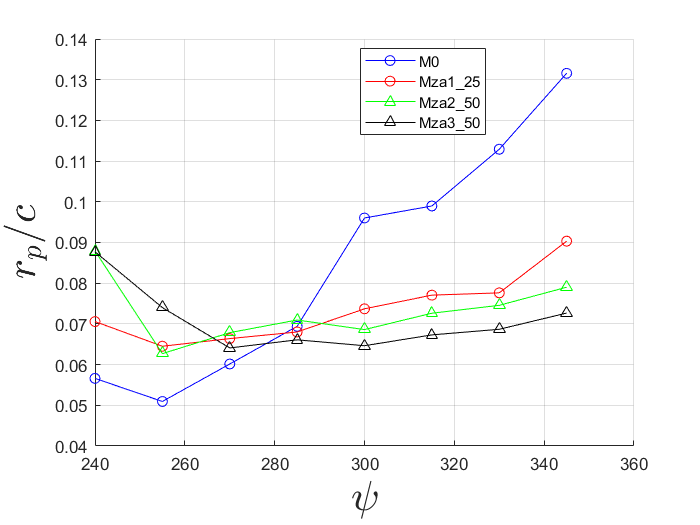
\includegraphics[width=0.7\textwidth]{figures/zonal_adapt_results/LEV/LEV_radius_vp}
	\caption{ Adaptive LES at $Re=40,000$: LEV size}
	\label{fig:zonal_LEV_radius}
\end{figure}

Figure \ref{fig:zonal_LEV_location} shows the location of the center of the LEV for different phases after it is ejected from the airfoil surface. 
It is observed that LEV formation for M0 mesh occurs closer to the geometric leading edge, as well as closer to the airfoil surface as compared to the other meshes.
For the initial phase of LEV location, Mza2\_nz50 and Mza3\_nz50 meshes show some differences, where Mza3\_nz50 mesh shows LEV formation closer to the airfoil surface and also closer to the geometric leading edge as compared to Mza2\_nz50 mesh.
After the initial phase, LEV paths for the finer meshes converge well, with Mza2\_nz50 and Mza3\_nz50 meshes showing a similar LEV path.


\begin{figure}[H]
	\centering
	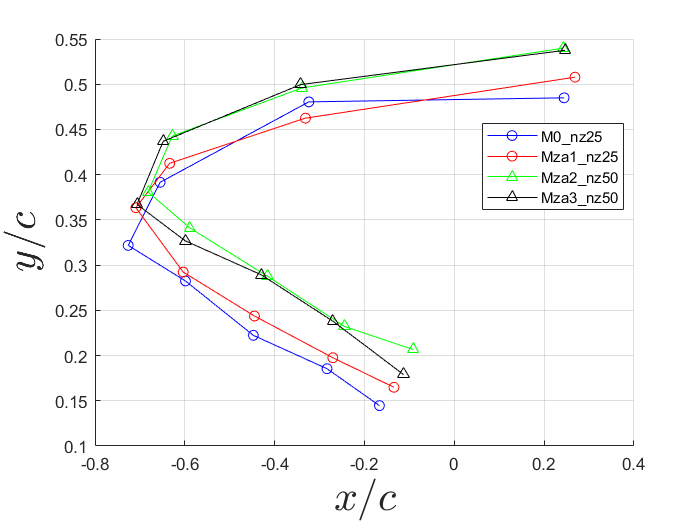
\includegraphics[width=0.75\textwidth]{figures/zonal_adapt_results/LEV/LEV_location}
	\caption{ Adaptive LES at $Re=40,000$: LEV position}
	\label{fig:zonal_LEV_location}
\end{figure}

Figure \ref{fig:zonal_utheta_LEV} shows the tangential/azimuthal velocity ($u_{\theta}$) profiles for the LEV from different meshes at 4 phases of $\psi = 240^\circ$,  $\psi = 270^\circ$ and  $\psi = 300^\circ$. 
Note that the tangential velocity is computed along multiple radial lines passing through the LEV center, and the mean tangential velocity over these radial lines is shown in Figure \ref{fig:zonal_utheta_LEV}, along with a 95\% confidence interval due to multiple radial lines.
The radial distance from the center of the LEV, $r$, is normalized by the LEV core radius $r_c$ of the finest mesh (Mza3\_nz50 mesh in this case) at that particular phase. 

For $\psi = 240^\circ$, max $u_\theta$ is achieved around $r/r_c = 0.6$ for M0\_nz25 mesh and around $r/r_c = 0.8$ for Mza1 mesh, 
For Mza2\_nz50 and Mza3\_nz50 meshes, the max $u_\theta$ is achieved at $r/r_c = 1$. Note that since $r$ is normalized with $r_c$ from Mza3\_nz50 mesh, max $r/r_c$ will always be 1 for Mza3\_nz50 mesh. 
Mean tangential velocity profile for both Mza2\_nz50 and Mza3\_nz50 meshes agree well along with the 95\% confidence interval. 
Also note the large thickness of the confidence interval band around the mean, which can be attributed to the LEV core being azimuthally asymmetric, since the LEV in this phase is close to the airfoil surface, as can be seen in Figure \ref{fig:vorticity_zonal_240}.

For $\psi = 270^\circ$, maximum $u_\theta$ is achieved around $r/r_c= 1$ for all meshes. 
M0\_nz25 and Mza1 meshes predict a lower tangential velocity as compared fto Mza2\_nz50 and Mza3\_nz50 meshes. 
Mean tangential velocity profile for Mza2\_nz50 and Mza3\_nz50 meshes agree well with each other, with Mza2\_nz50 mesh predicting slightly higher tangential velocity than Mza3\_nz50 mesh. 
The confidence interval for Mza3\_nz50 mesh lies within the confidence interval for Mza2\_nz50 mesh.

At $\psi = 300^\circ$, for Mza2\_nz50 and Mza3\_nz50, both the mean and confidence interval for the tangential velocity matches very well, apart for slight differences at higher $r/r_c$ values. 
Max $u_\theta$ for both these meshes is around $r/r_c= 1$.
Also note that the thickness/width of the confidence interval has reduced significantly as compared to the previous phases, showing that the LEV core is more azimuthally symmetric at this phase than the previous phases, as it is further away from the airfoil surface.
Mza1\_nz25 predicts a lower tangential velocity than the finer meshes, with max $u_\theta$ around $r/r_c= 1.1$. M0\_nz25 mesh predicts the lowest tangential velocity, and the max $u_\theta$ is not reached within $r/r_c= 1.1$.

\begin{figure}[H]
	\centering
	\begin{subfigure}[b]{0.475\textwidth}
	\centering
	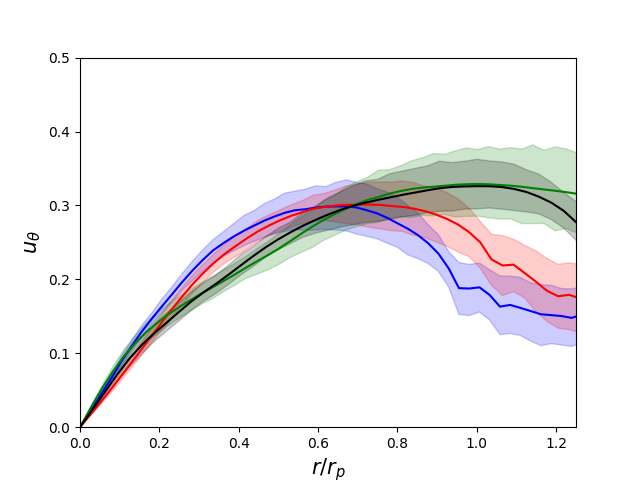
\includegraphics[width=1\textwidth]{figures/zonal_adapt_results/LEV/u_theta/phase_240.png}
	\caption{ $u_\theta$ at $\psi$ = $240^\circ$}
	\label{fig:zonal_utheta_240}
	\end{subfigure}
	\begin{subfigure}[b]{0.475\textwidth}
	\centering
	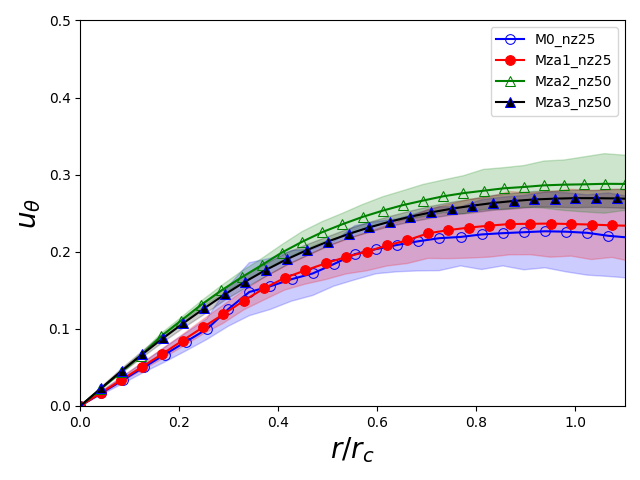
\includegraphics[width=1\textwidth]{figures/zonal_adapt_results/LEV/u_theta/phase_270.png}
	\caption{ $u_\theta$ at $\psi$ = $270^\circ$}
	\label{fig:zonal_utheta_270}
    \end{subfigure}
	\begin{subfigure}[b]{0.475\textwidth}
	\centering
	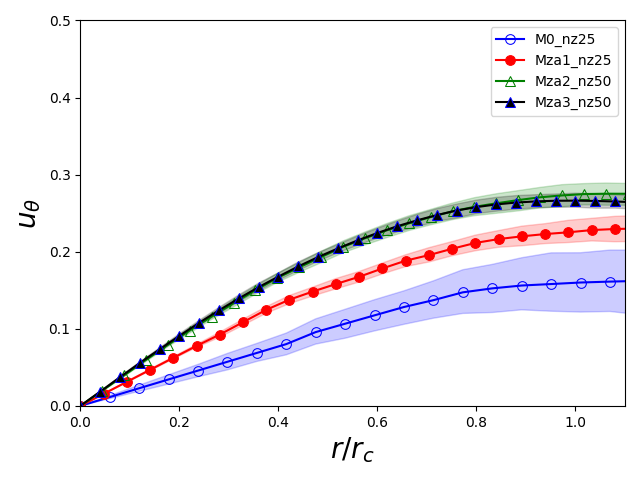
\includegraphics[width=1\textwidth]{figures/zonal_adapt_results/LEV/u_theta/phase_300.png}
	\caption{ $u_\theta$ at $\psi$ = $300^\circ$}
	\label{fig:zonal_utheta_300}
	\end{subfigure}
   	\caption{Adaptive LES at $Re=40,000$: LEV tangential velocity profile (including 95\% confidence interval)}
   	\label{fig:zonal_utheta_LEV}
\end{figure}

%TODO: location wrt ground is similar to Chapter 4. We don't look into it, since they don't add any more quanti info, and for brevity...

%TODO: Instead, we look into LEV tangential profiles and TI

Figure \ref{fig:zonal_TI_plots_LEV} shows the turbulence intensity profiles for LEV at 4 phases of $\psi = 240^\circ$, $\psi = 270^\circ$ and $\psi = 300^\circ$. 
Note that it is taken along multiple radial lines passing through the LEV center, in a similar fashion to tangential velocity profiles.

At $\psi = 240^\circ$, turbulence intensity for M0\_nz25 mesh increases with radial distance from center of LEV till about $r/r_c = 0.6$ and then starts to drop after this location.
Mza1 mesh follows a similar profile, with a less gradual drop in turbulence intensity for higher $r/r_c $ values.
Mza2\_nz50 and Mza3\_nz50 meshes agree reasonably well with each other, with both showing a higher turbulence intensity for higher $r/r_c$ values.


At phase $\psi = 270^\circ$, turbulence intensity increases for all meshes with increase in radial distance from the center of LEV.
Turbulence intensity is lowest overall for M0\_nz25 mesh, followed by Mza1\_nz25 mesh. Turbulence intensity for Mza2\_nz50 and Mza3\_nz50 meshes is the highest, and compare well with each other.

At phase $\psi = 300^\circ$, amongst all the meshes, M0\_nz25 mesh shows the highest turbulence intensity closer to the LEV center, till about $r/r_c = 0.25$, and lowest after this location.
Note that M0\_nz25 mesh fails to predict the trend in turbulence intensity as compared to other meshes.
Mza1\_nz25 mesh predicts a higher turbulence intensity as compared to the finer meshes, Mza2\_nz50 and Mza3\_nz50, till about $r/r_c = 0.25$, and lower after this location.
Turbulence intensity for Mza2\_nz50 and Mza3\_nz50 meshes agree well with each other. 


\begin{figure}[H]
	\centering
	\begin{subfigure}[b]{0.475\textwidth}
		\centering
		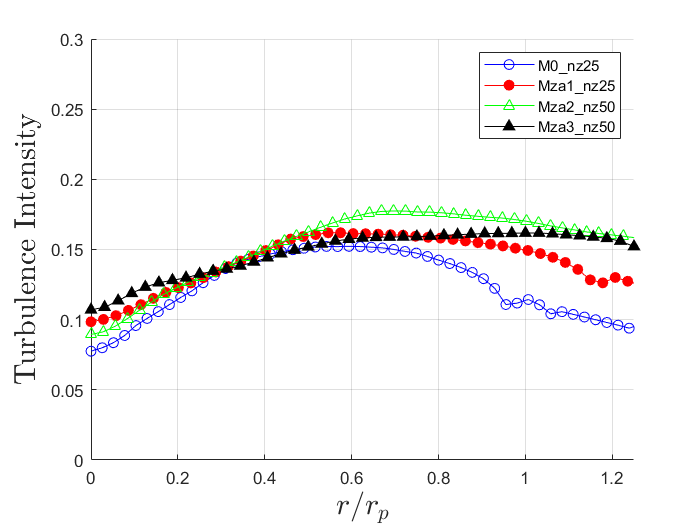
\includegraphics[width=1\textwidth]{figures/zonal_adapt_results/LEV/u_theta/TI_phase_240.png}
		\caption{$\psi$ = $240^\circ$}
		\label{fig:zonal_TI_240}
	\end{subfigure}
	\begin{subfigure}[b]{0.475\textwidth}
		\centering
		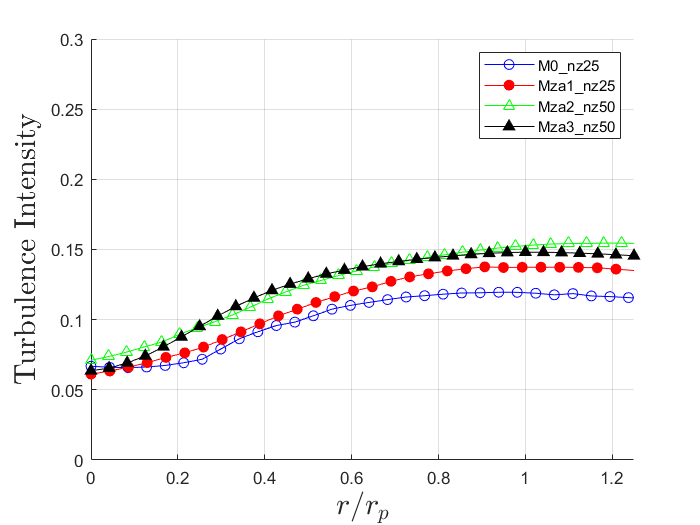
\includegraphics[width=1\textwidth]{figures/zonal_adapt_results/LEV/u_theta/TI_phase_270.png}
		\caption{$u_\theta$ at $\psi$ = $270^\circ$}
		\label{fig:zonal_TI_270}
	\end{subfigure}
	\begin{subfigure}[b]{0.475\textwidth}
		\centering
		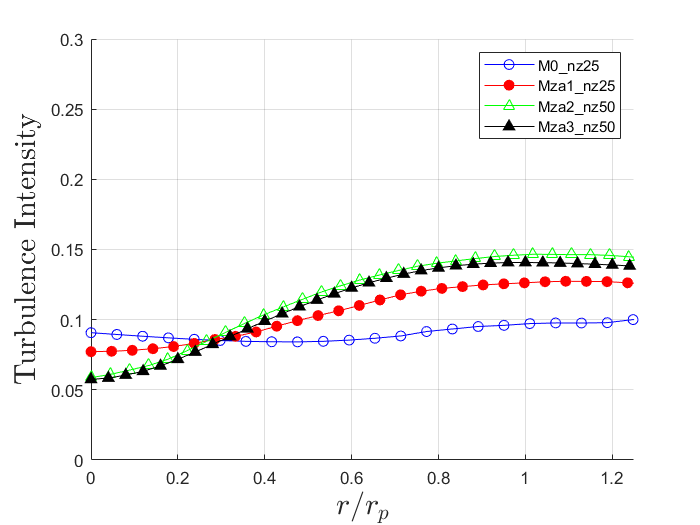
\includegraphics[width=1\textwidth]{figures/zonal_adapt_results/LEV/u_theta/TI_phase_300.png}
		\caption{$u_\theta$ at $\psi$ = $300^\circ$}
		\label{fig:zonal_TI_300}
	\end{subfigure}
	\caption{ Adaptive LES at $Re=40,000$: LEV turbulence intensity profiles}
	\label{fig:zonal_TI_plots_LEV}
\end{figure}

\subsubsection{Summary}
In summary, a thorough quantitative comparison of relevant quantities, such as spanwise vorticity, $C_p$ and LEV evolution and quantification, is performed for a series of adapted meshes. Mza2\_nz50 mesh compares well with Mza2\_nz100, Mza3\_nz50, and Mza3\_nz100 for all of the quantities considered above. This demonstrates mesh convergence and shows that the Mza2\_nz50 mesh is adequate for accurate LES for this case.